\documentclass{article}

% LTeX: language=fr
\usepackage[english,french]{babel}

\usepackage{graphicx} 
\usepackage{xcolor}
\usepackage{listings}
\usepackage[many,listings]{tcolorbox}
\tcbuselibrary{listingsutf8, skins}
\usepackage[colorlinks=true, linkcolor=blue, urlcolor=blue, citecolor=blue]{hyperref}

\usepackage[T1]{fontenc}

\definecolor{bgDark}{HTML}{3d3e4f}
\definecolor{strColor}{HTML}{81d6de}
\definecolor{numColor}{HTML}{9fbddf}
\definecolor{kwColor}{HTML}{f3afab}
\definecolor{opColor}{HTML}{89dcfd}
\definecolor{builtinColor}{HTML}{e07b00}
\definecolor{funcColor}{HTML}{b3c0e8}
\definecolor{textColor}{HTML}{ffffff}
\definecolor{commentGray}{HTML}{999999}
\definecolor{boxBorder}{HTML}{9999a1}

\definecolor{codebg}{HTML}{e4ebeb}
\definecolor{codefg}{HTML}{232938}


\lstdefinelanguage{myC}[]{C}{
  morekeywords={
    pragma,omp,parallel,atomic,reduction,num_threads,single,critical,
    schedule,dynamic,static,shared,private,firstprivate,default,barrier,
    nowait
  },
  otherkeywords={\#}
}


\lstdefinestyle{CStyle}{
  language=myC,
  backgroundcolor=\color{bgDark},
  basicstyle=\ttfamily\footnotesize\color{textColor},
  keywordstyle=\color{kwColor}\bfseries,
  identifierstyle=\color{textColor},
  commentstyle=\itshape\color{commentGray},
  stringstyle=\color{strColor},
  numberstyle=\color{bgDark},
  numbers=none,
  numbersep=6pt,
  showstringspaces=false,
  breaklines=true,
  breakatwhitespace=true,
  aboveskip=0pt,
  belowskip=0pt,
  frame=none,
  literate={\#}{{{\color{opColor}\#}}}1,
  emph={compute_first_line, get_selected_objects,malloc,
  omp_get_thread_num,free,main,printf,exit},
  emphstyle=\color{funcColor}\bfseries
}

% Boîte personnalisée pour encadrer le code C
\tcolorboxenvironment{lstlisting}{
  colback=bgDark,  % fond du listing
  colframe=boxBorder,  % bordure
  arc=3mm,  % arrondi
  outer arc=3.3mm,
  boxrule=0.8pt,  % épaisseur de la bordure
  left=5pt,
  right=5pt,
  top=5pt,
  bottom=5pt,
  enhanced,
  before skip=10pt,
  after skip=10pt,
}

\newtcbox{\inlinecode}{on line,
  colback=codebg,
  colupper=codefg,
  colframe=codebg,    % Même couleur que le fond → bordure invisible
  boxrule=0pt,        % Épaisseur bordure nulle
  arc=1mm,            % Arrondi léger
  top=0.4mm,
  bottom=0.4mm,
  left=1mm,
  right=1mm,
  box align=base,
  fontupper=\ttfamily\footnotesize,
}


\graphicspath{ {./images/} }

\begin{document}

\section{Explication du sujet}

Nous nous situons dans un environnement, une carte ou \textit{map} de ($100m \times 100m$) comme dans un jeu vidéo, dans laquelle il y a des obstacles, des individus, et un drone.
Le drone représente un point d'accès wifi, c'est-à-dire qu'il fournit du réseau à des utilisateurs.
Dans ce contexte, nous proposons de développer une intelligence artificielle (IA) capable de réaliser au minimum
les objectifs suivants:

\begin{itemize}
    \item \textbf{Maximiser} le débit fournit à tous les utilisateurs.
    \item Apprendre à \textbf{naviguer} (éviter les obstacles)
    \item Consommer le moins d'énergie possible (donc \textbf{atteindre son premier objectif le plus vite possible})
\end{itemize}    

\vspace{0.5cm}
Il y a donc trois axes à trainer pour le développement de la solution :
\begin{itemize}
    \item La partie simulation (monde physique en 3D).
    \item La partie apprentissage.
    \item La partie interface graphique (GUI), permettant de tester et comparer les résultats.
\end{itemize}

\begin{center}
    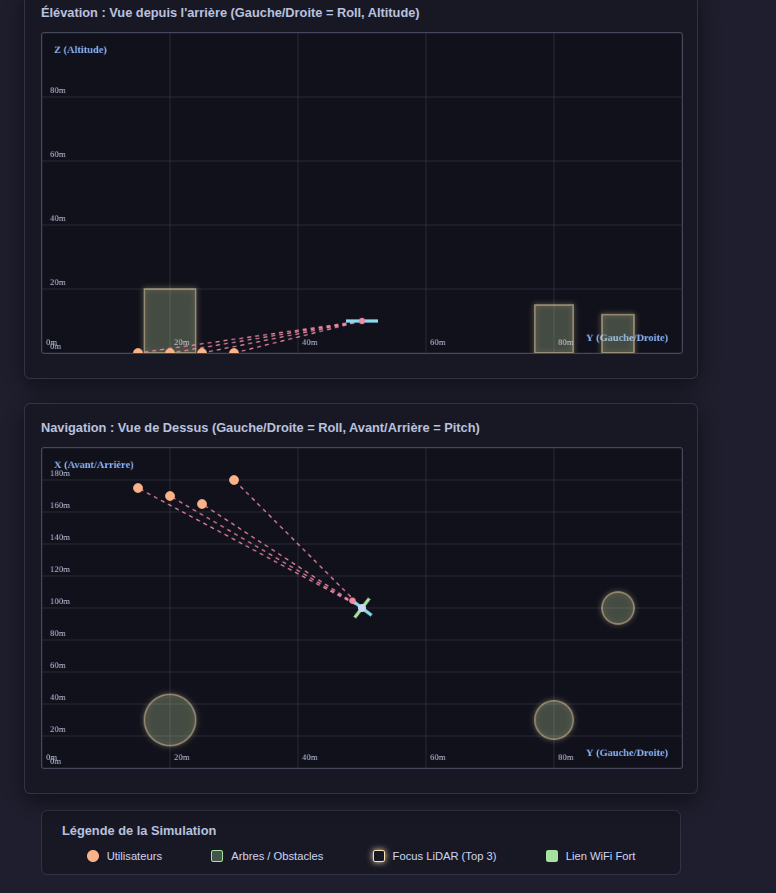
\includegraphics[width=0.5\textwidth]{images/simu.png}
\end{center}

\textbf{Hiérarchie des fichiers}
\begin{itemize}
    \item À chaque fois que nous parlerons de simulation physique,
    l'implémentation associée se trouvera dans les fichiers \texttt{simulation.c} et \texttt{simulation.h} (les .h sont dans \texttt{include}). 
    Certaines fonctions sont également dans \texttt{env.c}. En effet, le module \texttt{env} est un module qui fait le lien entre la simulation physique et l'apprentissage,
    c'est comment le drone voit la physique de son point de vue simplifié (il exécute uniquement des commandes moteurs telles que \texttt{ENGINE\_UP}).
    \item Tout ce qui est lié à l'apprentissage se trouve dans \texttt{model.c} et \texttt{model.h}. C'est là que se trouve l'IA.
    \item Tout ce qui est lié à l'interface graphique se trouve dans le sous-dossier \texttt{web}. Puisque l'interface graphique est \texttt{uniquement}
    \item liée à la simulation physique, les fonctions qui doivent envoyer des données à l'interface doivent se trouver dans \texttt{simulation.c}.
    \item Le reste (fonction de récompense, gestion des obstacles), est réparti entre \texttt{simulation} et \texttt{env}
\end{itemize}

\section{Apprentissage par renforcement}

Ici, nous introduisons et rappelons le principe de l'apprentissage par renforcement (RL), qui est la base de notre solution.
Le principe du RL est très simple, l'idée est que nous nous positionnons dans un environnement. 
Ce dernier est défini par la struct \texttt{world} dans \texttt{simulation.h}, c'est-à-dire que l'environnement est le monde réel.
Il a des individus, des obstacles, et des propriétés physiques (comme la gravité, etc.). Puisque pour le moment, \textbf{seul le drone} est associé
à un comportement physique (les utilisateurs sont immobiles, ce sont des points dans l'espace), les propriétés physiques appartiennent à
la structure \texttt{Drone}.

\begin{lstlisting}[style=CStyle]
typedef struct {
    Drone *drone;
    User *users;
    Obstacle3D *obstacles;
    int numUsers;
    int numObstacles;
    double width, height, depth;    // Dimensions de la carte. Attention, depth est la vraie hauteur ! (axe Z vers le haut)
} World;

\end{lstlisting}

\begin{lstlisting}[style=CStyle]
    typedef struct {
    double x, y, z; // Position
    double x_dot, y_dot, z_dot; // Vitesse lineaire
    double x_dot_dot, y_dot_dot, z_dot_dot; // Acceleration lineaire
    double phi, theta, psi; // Angles roll, pitch et yaw
    double phi_dot, theta_dot, psi_dot; // Derivees des angles
    double p, q, r; // Vitesse angulaire
    double p_dot, q_dot, r_dot; // Derivees des vitesses angulaires
    double omega[4]; // Vitesses de rotation des moteurs

    double target_thrust;
    double target_roll;
    double target_pitch;
    double target_yaw;

    PIDController pid_roll;
    PIDController pid_pitch;
    PIDController pid_yaw;

} Drone;
\end{lstlisting}

L'agent, c'est tout ce qui est lié au comportement du drone quand on lance une simulation.
Autrement dit, c'est un ensemble d'algorithmes qui, sans connaître l'environnement, 
vont devoir apprendre à interagir avec l'environnement de la bonne manière pour atteindre un objectif.
À chaque instant, l'agent observe l'état de l'environnement. Dans notre simulation, l'agent observe un nouvel état toutes 
les \textbf{0.01 secondes}. C'est l'intervalle de temps \texttt{dt}.
Il va devoir choisir des actions, et en fonction de ces actions, il va recevoir des récompenses ou des pénalités.
En prenant une action, l'agent arrive dans un nouvel état.

\vspace{0.5cm}

\textbf{Exemple : } Si l'agent choisit de se déplacer dans une direction, il va recevoir une récompense positive s'il se rapproche d'un utilisateur,
 et une pénalité s'il se rapproche d'un obstacle. Il arrive ensuite dans un nouvel état où il est soit plus proche d'un utilisateur, 
 ou bien plus proche d'un obstacle. Sa position a changé.
Il répète ce processus, et au fil du temps, il apprend à choisir les actions qui lui rapportent le plus de récompenses, c'est-à-dire les actions qui l'aident à atteindre son objectif.
Il cherche donc à \textbf{maximiser ses récompenses}. C'est ici le principe clé du projet.

\vspace{0.5cm}

\textbf{Dans toute la suite, on appelle}
\begin{itemize}
    \item $R(s, a)$ ou plus simplement $R$ la fonction de récompense. C'est-à-dire la récompense obtenue à l'instant $t$ en prenant l'action $a$ dans l'état $s$.
    \item $T(s, a, s')$ ou plus simplement $T$ la fonction de transition. C'est-à-dire l'état $s'$ dans lequel on arrive à l'instant $t+1$ en prenant l'action $a$ dans l'état $s$.
    \item On retiendra $T(s, a, s', r)$. On associe aussi la récompense obtenue en faisant cette transition.
    \item $S$ l'ensemble des états
    \item $A$ l'ensemble des actions
\end{itemize}
 
Remarque : $R$ et $T$ sont des fonctions, mais dans la pratique, on va représenter $R$ par un \texttt{double}, c'est la somme cumulée des récompenses obtenues en prenant l'action $a$ dans l'état $s$.
Pourquoi ? Car l'agent peut recevoir une pénalité de temps (s'il se déplace trop lentement), une pénalité de collision (si on se rapproche d'un obstacle),
 une récompense de proximité (si on se rapproche d'un utilisateur), etc. 
 Donc $R$ est la somme de toutes ces récompenses et pénalités.
$T$ est une structure en C qui contient les données associées.

\vspace{0.5cm}

On a dit que l'objectif \textbf{ultime} était de maximiser les récompenses.
Rien de plus simple, il faut maximiser le résultat de cette équation (\textbf{équation de Bellman}):
$$Q(s, a) = Q(s, a) + \alpha \left[R(s, a) + \gamma \sum_{s'} T(s, a, s') \max_{a'} Q(s', a') - Q(s, a)\right]$$.

\vspace{0.5cm}

\textbf{Détaillons chaque membre :}

$Q(s, a)$, c'est ce qu'on appelle une \textit{Q-value}, c'est la valeur de l'action $a$ dans l'état $s$. 
$Q$ est donc un vecteur qui contient la valeur de chaque action dans chaque état.
Attention, \textbf{ce n'est pas} la récompense obtenue en prenant l'action $a$ dans l'état $s$,
c'est la somme de la récompense immédiate $R(s, a)$ et du gain future que l'agent espère obtenir, soit
 $\gamma \sum_{s'} T(s, a, s') \max_{a'} Q(s', a') - Q(s, a)$.
En résumé, $Q(s, a)$ est une estimation temporelle de la récompense.

\vspace{0.5cm}

La somme $\sum_{s'} T(s, a, s') \max_{a'} Q(s', a')$ représente la récompense future, 
c'est-à-dire la récompense qu'on peut espérer obtenir en prenant l'action $a$ dans l'état $s$ \textbf{immédiatement} :
($T(s, a, s')$) et en suivant la meilleure politique par la suite 
(c'est-à-dire en choisissant les actions qui maximisent $Q(s', a')$ dans les états futurs $s'$).

\vspace{0.5cm}

La différence $R(s, a) + \gamma \sum_{s'} T(s, a, s') \max_{a'} Q(s', a') - Q(s, a)$ représente l'erreur de prédiction.
Actuellement, la "valeur" de l'action $a$ est $Q(s, a)$. Le \textbf{gain} qu'on espère obtenir, c'est la différente entre la cible
(ce qu'on vise dans le futur) et la valeur actuelle. C'est cette différence qu'on va essayer de minimiser au fil du temps, 
pour que $Q(s, a)$ converge vers la valeur réelle de l'action $a$ dans l'état $s$.

\vspace{0.5cm}

Mais comment on obtient $Q(s, a)$ puisque que nous n'avons pas encore simulé le futur ? C'est là que le \textbf{Q-learning} entre en jeu.
En fait, au début de l'apprentissage, on initialise $Q(s, a)$ à 0 pour tous les états $s$ et toutes les actions $a$.
La première fois qu'on fera le calcul, on aura $Q(s, a) = R(s, a)$ donc la récompense immédiate.
Ensuite, nous aurons $R$ + $R'$, puis $R$ + $R'$ + $R''$, etc. Bien sûr, ici, nous simplifions. Cela signifique
que $R$, $R'$, \dots sont à la fois la récompense immédiate et le gain (erreur de prédiction).
Finalement, nous avons $Q(s, a) = Q(s, a) + \dots$, car il se met à jour.
Donc mentionné plus haut, $Q(s, a)$ va converger vers la valeur réelle de l'action $a$ dans l'état $s$.
Il faut le voir un peu comme un effet "récursif".

\vspace{0.5cm}

L'hyperparamètre $\alpha$ est le taux d'apprentissage, soit la confiance que l'on accorde à notre valeur.
Nous pondérons en fait la valeur obtenue par ce facteur.
L'hyperparamètre $\gamma$ est appelé le \textit{discount factor}, il permet de donner plus ou moins d'importance aux récompenses futures par rapport aux récompenses immédiates.
On remarque que si $gamma$ = 0, l'équation devient $Q(s, a) = R(s, a)$, l'agent ne se soucie que des récompenses immédiates.
Si $\gamma$ = 1, l'agent se soucie autant des récompenses futures que des récompenses immédiates.
Nous, on prendra $gamma$ = 0.99 car le problème est très complexe.

\vspace{0.5cm}

\textbf{Algorithme du Q-learning}

\vspace{0.5cm}

Une notion \textbf{importante} est la notion d'\textbf{exploration vs exploitation}.
L'idée est que l'agent doit trouver un équilibre entre l'exploration de nouvelles actions et l'exploitation des actions qu'il connaît déjà.
Si l'agent exploite toujours les actions qu'il connaît déjà, il risque de se retrouver coincé dans une solution sous-optimale (comme un mauvais minimum local en \textit{Deep Learning}).
Si l'agent explore toujours de nouvelles actions, il risque de ne jamais converger vers une solution optimale.


\begin{lstlisting}[style=CStyle]
 
QLearning <- function(states, actions, T, R, max_epochs = 100, max_step = 10, epsilon = 0.1) {
  
  // Initialisation de la table Q
  Q <- [[0]]
  
  // On sauvegarde l'etat initial
  initial_state <- states[1]
  
  // Les epochs, c'est le nombre de fois qu'on va faire l'apprentissage complet, cad le nombre de fois qu'on va faire le processus d'apprentissage du debut a la fin.
  for (epoch in 1:max_epochs) {
    state <- initial_state // A chaque epoch, on recommence a l'etat initial
    
    // Le steps, c'est le nombre d'actions et d'etat que l'agent va virve dans la simulation physique pendant une epoch.
    for (step in 1:max_step) {
      
      // On tire un nombre aleatoire pour svaoir si on va explorer ou exploiter
      if (runif(1) < epsilon) {
        action <- rand(nbaction) // On explore
      } else {
        action <- which.max(Q[state, ]) // On exploite, on prend l'action qui a la meilleure Q-value dans l'etat actuel
      }
      
      new_state <- T(state, action)  // C'est un step de la simulation physique, donc de l'environnement, appele envStep dans le code
      reward <- R(state, action) // getReward
      
      // Mise a jour de la table Q selon l'equation de Bellman
      Q[state, action] <- Q[state, action] + (reward + gamma * max(Q[new_state, ]))
      
      state <- new_state
    }
  }
  return (Q)
}
   
\end{lstlisting}


\section{Q-Network}

Le problème du \textit{Q-learning}, c'est que si on a un grand nombre d'états et d'actions, la table devient très grande et difficile à gérer.
Et c'est le cas ici. En effet, il y a un nombre infini d'états, car les positions sont des nombres flottants. De plus, nous définissions également l'état du drone par sa vitesse,
son orientation, sa vitesse angulaire... et il doit prédire la prochaine action à prendre en fonction de toutes ces informations.

\begin{lstlisting}[style=CStyle]
typedef struct {
    double x, y, z; // Position
    double x_dot, y_dot, z_dot;
    double x_dot_dot, y_dot_dot, z_dot_dot;
    double phi, theta, psi;
    double phi_dot, theta_dot, psi_dot;
    double p, q, r; // Vitesse angulaire
    double p_dot, q_dot, r_dot;
    double omega[4]; // Vitesses de rotation des moteurs

    ...
} Drone;
\end{lstlisting}

C'est pour cette raison qu'on va utiliser un réseau de neurone pour approximer la fonction $Q$.
Cette technique s'appelle le \textbf{Deep Q-learning}.
Remplaçons dans notre équation $Q$ par $Q_\text{N}$ (pour Q-Network), qui est un réseau de neurone qui prend en entrée le \textbf{vecteur d'état}
(ensemble des données physiques du monde) et qui sort un vecteur de \textit{Q-values} pour chaque action possible :
$$Q_\text{N}(s) = [Q(s, a_1), Q(s, a_2), ..., Q(s, a_n)]$$
Du coup, si on veut savoir quelle action prendre, nous devons simplement faire un \texttt{argmax} sur ce vecteur de sortie.

Sur le schéma ci-dessous, le vecteur d'entrée $X$, correspond au vecteur d'état, et le vecteur de sortie $Y$ correspond
à $Q_\text{N}(s)$, le vecteur de \textit{Q-values} pour chaque action.

\begin{center}
    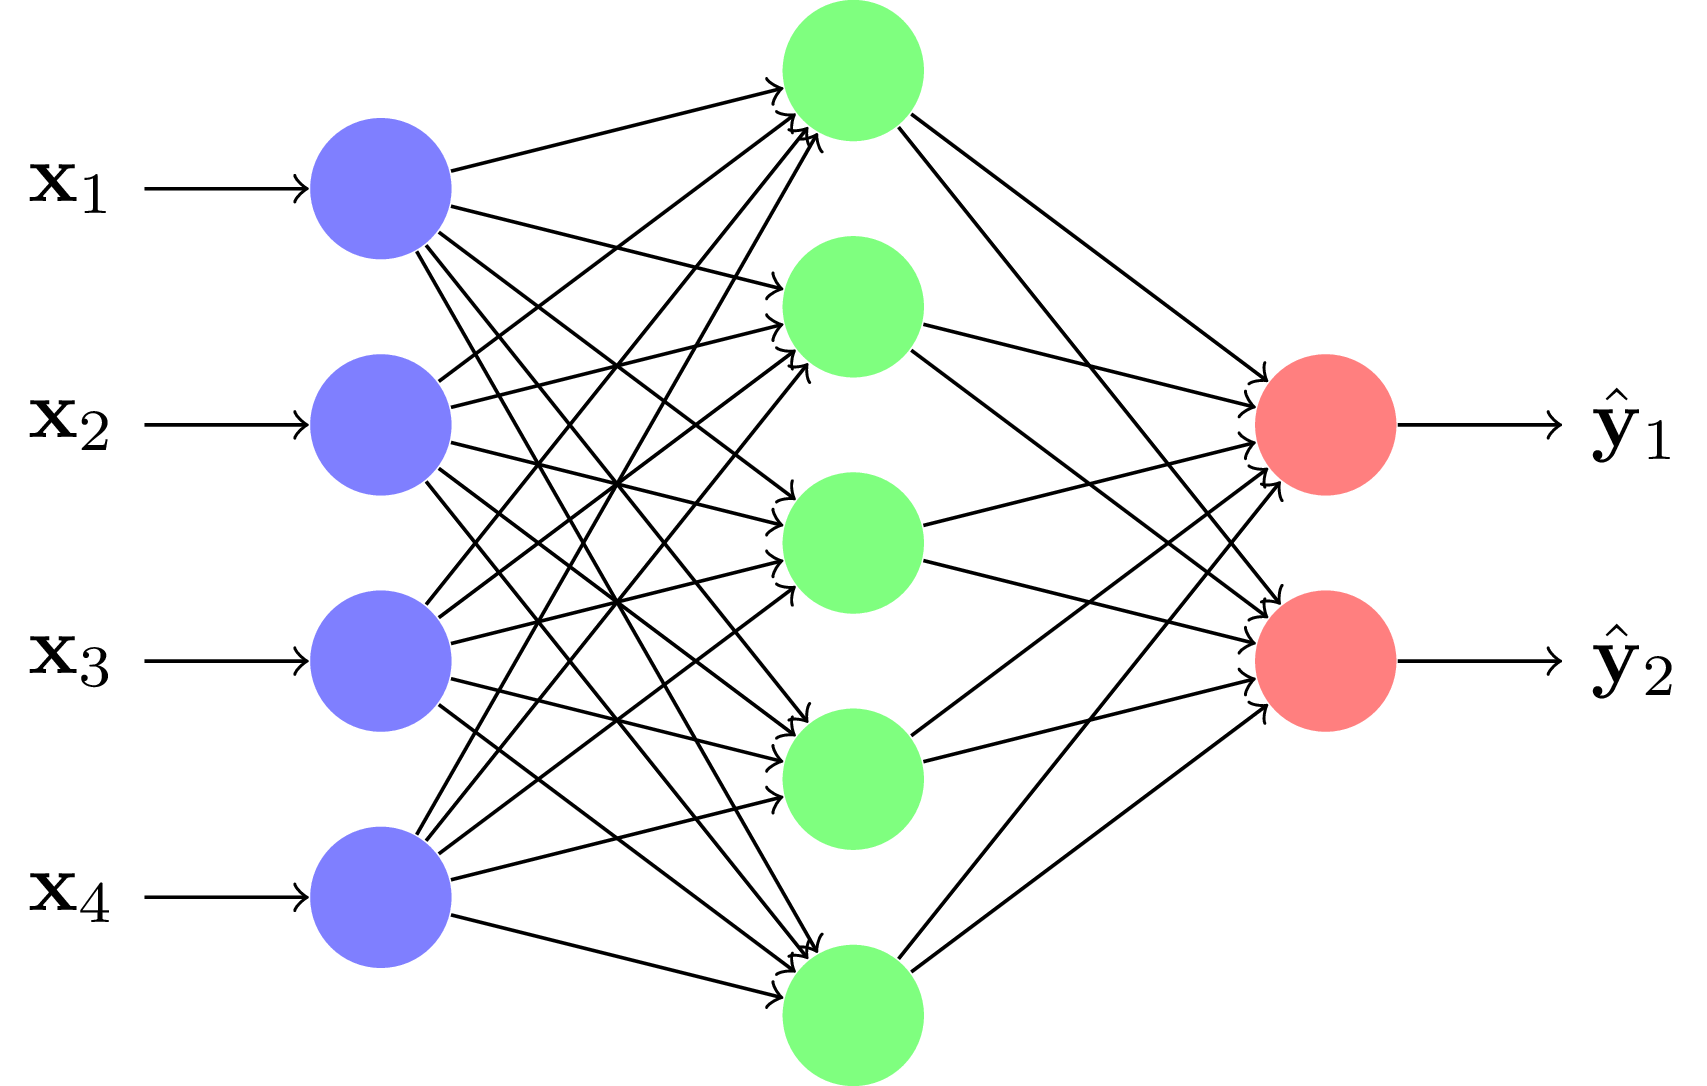
\includegraphics[width=0.5\textwidth]{images/nn.png}
\end{center}

Les sections qui suivent présentent des extensions ainsi que des détails d'implémentation, pour résoudre toutes les \textbf{difficultés} qui vont s'accumuler à cause de la nature
du problème (espace continu).

\section{Target Network}

Maintenant, l'équation change un peu. Car c'est le réseau de neurone qui possède un \textit{learning rate} ($\alpha$) 
et qui va faire une descente de gradient pour minimiser l'erreur de prédiction.
L'équation se "simplifie".

Nous réécrivons l'équation de \textbf{}Bellman pour le \textit{Deep Q-learning}.
$$Q_\text{N}(s, a) = R(s, a) + \gamma \sum_{s'} T(s, a, s') \max_{a'} Q_\text{N}(s', a')$$

En se référant à l'image ci-dessus, nous rappelons que lorsqu'un un réseau de neurone s'entraîne, il fait pour chaque \textit{epoch} une descente de gradient :
\begin{itemize}
    \item Il fait une propagation avant pour prédire $Q_\text{N}(s, a)$ : ce membre apparaît toujours dans le réseau de neurone,
    il est seulement simplifié dans l'algorithme général d'apprentissage par renforcement.
    \item Il calcule l'erreur entre $Q_\text{N}(s, a)$ et $R(s, a) + \gamma \sum_{s'} T(s, a, s') \max_{a'} Q_\text{N}(s', a')$.
    \item Il fait une propagation arrière pour mettre à jour les poids du réseau afin de diminuer cette erreur.
\end{itemize}

\vspace{0.5cm}

Le problème auquel nous sommes confrontés, c'est qu'une \textit{backpropagation} modifie les poids, donc elle modifie la valeur de $Q_\text{N}(s, a)$ elle-même, et en conséquence,
$Q_\text{N}(s', a')$ change pour la prochaine itération, ce qui veut dire que l'action optimale pour l'état $s'$ change à chaque itération.
Le réseau ne peut pas converger.
C'est comme si notre objectif en athlétisme était d'atteindre la ligne d'arrivée, mais à chaque fois que nous faisons un pas, 
cette ligne d'arrivée se déplace de la même distance que nous, il est impossible de l'atteindre.

\vspace{0.5cm}

Pour régler ce problème, nous utilisons une technique appelée \textbf{Target Network}.
Nous retenons à présent deux réseaux de neurones, $Q_\text{N}$ et $Q_\text{T}$. $Q_\text{N}$ est le réseau de neurone principal qui est mis à jour à chaque itération, 
et $Q_\text{T}$ est un réseau de neurone "cible" qui est une copie de $Q_\text{N}$ mais qui n'est mis à jour que tous les $C$ épisodes (par exemple tous les 10 épisodes).
Autrement dit, notre cible reste fixe pendant un certain temps, nous savons alors où aller et comment l'atteindre, puis elle bouge. Cependant, nous arrivons
à la rattraper sur le long terme car nous avons le temps de nous adapter.
Dans le code, la synchronisation a lieu tous les \texttt{networks\_update\_freq}.

\vspace{0.5cm}

Équation \textbf{finale} à résoudre :
$$Q_\text{N}(s, a) = R(s, a) + \gamma \sum_{s'} T(s, a, s') \max_{a'} Q_\text{T}(s', a')$$

\section{Replay Buffer}

Maintenant, un autre problème émerge dû à la nature continu de notre système. 
Dans le \textit{Q-Learning} classique, on choisit une action, on observe le nouvel état, et on met à jour la table. 
Ici si on fait ça, on va avoir un problème de corrélation des données.

\vspace{0.5cm}

\textbf{Exemple :}
On a dit que chaque pas de la simulation dans le monde physique correspond à $dt = 0.01$s.
Si à l'instant t, le drone est en ($x = 10$, $y = 10$), à l'instant $t + 0.01$, il est en ($x = 10.01$, $y = 10$).
Ces deux états sont quasi identiques. Si on entraîne le réseau dessus, il va \textit{overfitter} sur cette trajectoire et ne pas apprendre à voler.
En fait ça peut même être pire, car la différence dans le calcul de l'erreur (\textit{gradient descent}) peut être tellement faible 
que nous serons confrontés au problème du \textit{vanishing gradient}. Tous les poids vserons remis à $0$ à cause de cette corrélation des données.

\vspace{0.5cm}

Ici la solution, consiste à utiliser un \textbf{Replay Buffer}.
Le principe est de stocker les transitions, c'est-à-dire les tuples $(s, a, r, s')$ dans un \textbf{buffer circulaire} de taille fixe (par exemple 25 000).
À chaque fois que l'agent fait une action, on stocke la transition dans ce buffer.
À chaque fois que l'on veut prédire la prochaine action, on ne prend pas la transition la plus récente, 
mais on tire aléatoirement un \text{mini-batch} (ex : $64$) de transitions dans ce buffer 
afin que le réseau apprenne sur un mélange de situations passées.

Voici la structure que nous obtenons :

\begin{lstlisting}[style=CStyle]

typedef struct {
    double state[NB_STATES];      // Etat avant l'action
    EngineAction action;          // Action qu'on prend
    double reward;                // Recompense qu'on obtient
    double next_state[NB_STATES]; // Prochaine etat dans lequel on se trouve
    int next_state_terminal;      // Est-ce que le prochain etat est terminal (voir Env) ?
    int flag;                     // Utilise pour savoir si une donnee est deja tiree pour un batch (voir ReplayBuffer)
    double td_error;              // Utilise pour modifier les probabilites des tirages aleatoire (ReplayBuffer)
} Transition;

typedef struct {
    Transition *buffer; // Tableau alloue dynamiquement pour memoriser les transitions
    int capacity;       // Capacite max du buffer
    int size;           // Taille actuelle du buffer
    int head;           // Index d'insertion (buffer dynamique)
} ReplayBuffer;

typedef struct s_rl_model {
    NeuralNetwork *q_network;       // Reseau principa
    NeuralNetwork *target_network;  // Reseau cible
    Env *env;                       // Environnement
    ReplayBuffer *memory;           // Memoire pour l'Experience Replay
    Config config;                  // Config avec hyperparametres

    int batchSize;                  // Taille des batchs pour les reseaux de neurones
    double learningRate;            // Pour l'entrainement du reseau de neurone
    double decay;                   // Decay pour le learning rate du reseau de neurone
    int networks_update_freq;       // Frequence de synchronisation des deux reseaux (ex: 1000 steps)
    int step_count;                 // Compteur pour savoir quand synchroniser
    char *path;                     // Chemin de sauvegarde
    ...
} DQNModel;
\end{lstlisting}

\section{Fonctions DeepQLearning et updateNetworks}

\vspace{0.5cm} 

L'algorithme complet du \textit{DeepQLearnig} est disponible dans \texttt{model.c}.
Nous avons déjà parlé tout à l'heure, lorsque l'on entraine un réseau de neurones classique,
on utilise des \texttt{inputs} et des \texttt{expecteds\_outputs}. Il faut en effet savoir ce que l'on souhaite obtenir
pour calculer l'erreur.

\vspace{0.5cm}

Puisque nous n'avons pas de données d'entraînement (comme des images annotées pour la classification d'images), 
nous allons construire nos données d'entraînement à partir des transitions stockées dans le replay buffer.

\vspace{0.5cm}

Voici les étapes permettant de construire ce vecteur.

\begin{itemize}
    \item On tire un mini-batch de transitions dans le replay buffer : $\{(s, a, r, s')\}$.
    \item Une première prédiction avec le réseau de neurone principal $Q_\text{N}$ pour tous les états $s$ du mini-batch, 
    nous donne un vecteur de \textit{Q-values} pour chaque état : $Q_\text{N}(s) = [Q(s, a_1), Q(s, a_2), ..., Q(s, a_n)]$.
    \item Une deuxième prédiction avec le réseau de neurone cible $Q_\text{T}$ pour tous les états $s'$ du mini-batch, 
    nous donne un vecteur de \textit{Q-values} pour chaque état futur : $Q_\text{T}(s') = [Q(s', a_1), Q(s', a_2), ..., Q(s', a_n)]$.
    \item Nous construisons le vecteur d'outputs attendus pour chaque transition du mini-batch, en copiant d'abord le résultat de
    $Q_\text{N}(s)$. En effet, les autres valeurs de $Q_\text{N}(s, a')$ pour $a' \neq a$ \textbf{ne doivent pas}
    changer puisque le drone n'a choisi qu'une seule action à cet instant. Il ne faut pas effacer ses autres connaissances.
    Puis pour chaque transition $(s, a, r, s')$ du batch, on calcule la cible de la manière suivante :
    \begin{itemize}
        \item Si $s'$ est un état terminal, la cible est simplement $r$
        \item Sinon, la cible est $r + \gamma \max_{a'} Q_\text{T}(s', a')$
    \end{itemize}
    \item On met à jour la valeur de $Q_\text{N}(s, a)$ (donc de l'action réellement choisie) dans le vecteur d'outputs attendus avec la "nouvelle" meilleure action qui doit la remplacer,
     tandis que les autres valeurs restent inchangées comme précisé précédemment.
\end{itemize}


\section{Le Frame Skipping}

Bien que nous ayons réglé les problèmes de corrélation des données avec le replay buffer, nous avons toujours
 un problème de corrélation temporelle.
\textbf{Résumé rapide} des solutions mises en place jusqu'à présent :

\begin{itemize}
    \item On veut maximiser les récompenses du drone avec une équation théorique.
    \item Comme on a un espace continue, on prédit l'action que l'on va prendre avec un réseau de neurones.
    \item À cause de la mise à jour des poids et des gradients, nous devons utiliser un deuxième réseau qui sert d'objectif temporaire à atteindre et permettre la convergence.
    \item Mais à cause de la nature du problème, nous avons des problèmes de corrélation de données (effets très similaires sur un instant très petit quelque soit l'action), 
    donc on utilise un \textit{replay buffer} pour mélanger les données.
    \item Reste un problème de corrélation temporelle...
\end{itemize}


Dans notre simulation, nous avons précisé que l'agent observe un nouvel état toutes les $0.01$ secondes, 
c'est-à-dire que le drone fait une action toutes les $0.01$ secondes.
Mais en réalité, au bout de $0.01$ secondes, le drone ne voit pas encore les effets de son action.
Pour rappel, nous avons une vraie simulation physique 3D avec des forces de poussées, du tangage, etc.
Comme la poussée possède une certaine durée réelle, il faut un certain temps pour que le drone atteigne sa future position avec la vitesse \textbf{imprimée} par ce mouvement.
En résumé, le temps est discrétisé mais les actions ne le sont pas \textbf{par rapport au temps}.

\vspace{0.5cm}

Pour régler ce problème, on utilise une technique appelée \textbf{Frame Skipping}.
Au lieu de faire une action à chaque pas de temps ($0.01$s), on va faire une action tous les $k$ pas de temps
(par exemple tous les $4$ pas de temps, soit tous les $0.04$s).
Pendant les pas de temps intermédiaires, on va répéter la même action, et on va accumuler les récompenses obtenues durant ces pas de temps intermédiaires.
En conséquence, nous réduisons la corrélation temporelle, et permettons ainsi au drone \textbf{d'observer} les effets de son action avant de devoir en choisir une nouvelle.

\vspace{0.5cm}

L'algorithme présent dans le fichier \texttt{env.c} est le suivant :

\begin{lstlisting}[style=CStyle]
void envStep(Env *env, double *next_state, double *reward, int *is_terminal, int action_idx) {
    World *w = env->physical_world;
    double accumulated_reward = 0.0;
    int crashed = 0;

    handleCommand(w->drone, action_idx);

    // On laisse le drone executer l'action choisie pendant FRAME_SKIP iterations physiques
    for (int i = 0; i < FRAME_SKIP; i++) {
        physicsStep(w, DT);
        crashed = isDroneCrashed(w);
        accumulated_reward += getReward(env);
        if (crashed) break;
    }

    getStateVector(env, next_state);

    double final_reward = accumulated_reward / FRAME_SKIP; 

    if (crashed) { final_reward -= 100.0; }
    *reward = final_reward; 
    *is_terminal = crashed;
}
\end{lstlisting}


\section{Grid Density Mapping}

Une notion importante pour la fonction de récompense et la construction du vecteur d'état, 
c'est la notion de \textbf{Distribution Spatiale}. Revenons un peu sur l'architecture d'un réseau de neurones.

Cela est évident, mais pour faire une prédiction, le réseau de neurone doit prendre en entrée un vecteur 
de \textbf{taille fixe}, et doit sortir un vecteur de taille fixe.
Le vecteur sortant de taille fixe, nous l'avons déjà, c'est l'ensemble des actions possibles, qui est défini dans \texttt{simulation.h} par l'énumération suivante :

\begin{lstlisting}[style=CStyle]
 typedef enum {
    ENGINE_IDLE = 0,
    ENGINE_UP,
    ENGINE_DOWN,
    ENGINE_PITCH_LEFT,
    ENGINE_PITCH_RIGHT,
    ENGINE_ROLL_LEFT,
    ENGINE_ROLL_RIGHT,
    ENGINE_YAW_LEFT,
    ENGINE_YAW_RIGHT
} EngineAction;
\end{lstlisting}

\vspace{0.5cm}

Par contre, pour le vecteur entrant, c'est plus compliqué. En effet, l'état du drone est défini par sa position, sa vitesse, son orientation, etc.
Mais il y a aussi les utilisateurs, et les obstacles, et il peut y en avoir en nombre variable. Ils peuvent aussi être à des positions différentes à chaque instant.
Nous ne pouvons pas simplement construire un vecteur d'état contenant la position de chaque utilisateur et de chaque obstacle, car ce vecteur aurait une taille variable.
Il serait aussi très grand, puisque si on a $100$ utilisateurs, on aurait un vecteur de $300$ dimensions uniquement pour les utilisateurs ($x$, $y$, $z$ pour chaque utilisateur), et pareil pour les obstacles.

\vspace{0.5cm}

On veut donc 
\begin{itemize}
    \item \textbf{1.} Savoir combien il y a d'utilisateurs dans la carte
    \item \textbf{2.} Connaître la position de ces utilisateurs.
    \item \textbf{3.} Obtenir ces informations avec un evecteur de taille fixe
\end{itemize}

Compter les utilisateurs est simple, il suffirait un seul entier qui contient cette information.
Mais cela ne nous dit pas où ils sont, et ce n'est pas suffisant pour la fonction de récompense.
Autrement dit, le réseau ne peut pas faire la corrélation entre le nombre stocké dans cette variable d'état
et la position des utilisateurs en temps-réel, il ne peut donc pas apprendre à se rapprocher d'eux pour maximiser le débit.

\vspace{0.5cm}

\textbf{Par contre}, si on prend \textbf{plusieurs} compteurs, magiquement, le réseau va se débrouiller tout seul.
En fait, avoir plusieurs compteurs, c'est comme avoir un vecteur d'état de taille $N$ compteurs.
$$\text{state} = \begin{bmatrix}
\text{n}_1 \\
\text{n}_2 \\
\vdots \\
\text{n}_N
\end{bmatrix}$$

C'est aussi avoir une matrice dans laquelle nos $N$ compteurs sont répartis en $k$ lignes et $k$ colonnes :
$$\text{state} = \left[ \begin{array}{cccc}
\text{n}_1 & \text{n}_2 & \cdots & \text{n}_k \\
\text{n}_{k+1} & \text{n}_{k+2} & \cdots & \text{n}_{2k} \\
\vdots & \vdots & \ddots & \vdots \\
\text{n}_{(k-1)k+1} & \text{n}_{(k-1)k+2} & \cdots & \text{n}_{k^2}
\end{array} \right]$$

Au final, cela revient à diviser notre carte en une grille de $k \times k$ cellules, et chaque compteur va compter le nombre d'utilisateurs dans sa cellule.
C'est le principe de la \textbf{Distribution Spatiale}.
Dans notre cas, la variable \texttt{GRID\_SIZE} vaut $4$, donc nous avons $16$ cadrants. Chaque case est comme un pixel d'une image basse résolution, 
et la valeur de ce pixel représente le nombre d'utilisateurs dans cette case.

\vspace{0.5cm}

Si nous choisissons $4$ utilisateurs, le réseau aura en entrée une matrice (\textit{HeatMap}) ressemblant à cela :

$$\text{state} = \left[ \begin{array}{cccc}
\text{0.0} & \text{0.0} & \text{0.0} & \text{0.0} \\
\text{0.25} & \text{0.0} & \text{0.25} & \text{0.0} \\
\text{0.0} & \text{0.25} & \text{0.0} & \text{0.25} \\
\text{0.0} & \text{0.0} & \text{0.0} & \text{0.0}
\end{array} \right]$$

\vspace{0.5cm}

Chaque valeur est normalisée par le nombre total d'utilisateurs, donc elle est comprise entre 0 et 1, 
et elle représente la densité d'utilisateurs dans cette cellule.
Le réseau voit immédiatement où sont les zones de forte concentration humaine.
Il ne faut \textbf{pas une trop grosse grille} pour pas rajouter trop d'états,
sinon il faut également rajouter des couches de neurones, l'entraînement devient plus long et le réseau a plus de mal à apprendre.

\vspace{0.5cm}

L'algorithme est alors le suivant. On suppose que le drone sait où sont les utilisateurs.
Cela est acceptable dans le sens où dans la réalité, un drone peut détecter les utilisateurs grâce à leur signal wifi,
et il peut estimer leur position grâce à la force du signal.
Il itère donc sur chaque \textit{user} en regardant sa position, il calcule quel est \textbf{l'index} de la cellule
(c'est la position de l'utilisateur divisée par la taille d'une cellule) et il incrémente le compteur de la cellule correspondante.
Il place cette valeur dans le tableau \texttt{state} (qui sera le vecteur d'entrée du réseau).

\vspace{0.5cm}

Pour rappel, notre tableau d'entrée du réseau ne contient pas seulement ces informations, mais aussi toutes
les caractéristiques physiques du drone (position, vitesse, orientation, etc.). Ici on ne fait que le compléter
pour améliorer l'apprentissage du drone.



\begin{lstlisting}[style=CStyle]
static void fillUsersGrid(Env *env, double *state_out) {
    World *w = env->physical_world;

    int num_cells = GRID_SIZE * GRID_SIZE;
    for (int i = 0; i < num_cells; i++) state_out[i] = 0.0;

    for (int i = 0; i < w->numUsers; i++) {
        int cell_x = (int)(w->users[i].x / (w->width / GRID_SIZE));
        int cell_y = (int)(w->users[i].y / (w->height / GRID_SIZE));

        if (cell_x < 0) {cell_x = 0;} if (cell_x >= GRID_SIZE) {cell_x = GRID_SIZE - 1;}
        if (cell_y < 0) {cell_y = 0;} if (cell_y >= GRID_SIZE) {cell_y = GRID_SIZE - 1;}

        state_out[cell_y * GRID_SIZE + cell_x] += 1.0;
    }

    for (int i = 0; i < num_cells; i++) {
        if (w->numUsers > 0) state_out[i] /= w->numUsers;
    }
}
\end{lstlisting}

\section{Capteur LiDAR pour les obstacles}

Pour les obstacles, on ne peut pas supposer connaître leur position, car dans la réalité, 
un drone ne possède pas naturellement de cartographie de l'environnement avec la position de chaque arbre, etc. 
Il doit détecter les obstacles grâce à des capteurs comme le LiDAR.
Le LiDAR envoie des rayons dans toutes les directions, et mesure le temps que mettent ces rayons à revenir après avoir touché un obstacle, 
ce qui permet de construire une carte de son environnement immédiat.
On suppose alors que le drone est capable de détecter les $3$ obstacles les plus proches.
On insère leurs positions dans le vecteur d'état, après les compteurs de la grille des utilisateurs.
Tous ces algorithmes sont implémentés dans le fichier \texttt{env.c}.

\section{Curriculum Learning}

Le \textit{curriculum learning} est une extension légère apportée au \textit{Deep Q-learning} pour améliorer la capacité de généralisation du drone.
L'idée sous-jacente est d'entraîner l'agent sur des tâches de plus en plus difficiles.
Lorsque l'on réinitialise l'environnement au début de chaque \textit{epoch}.
\begin{itemize}
    \item De $0$ à $200$ \textit{epochs}, on peut garder la même configuration d'utilisateurs et d'obstacles, pour que le drone puisse apprendre à voler et à se rapprocher des utilisateurs.
    \item De $200$ à $500$ \textit{epochs}, on peut introduire une légère randomisation, pour que le drone puisse apprendre à s'adapter à des environnements légèrement différents.
    \item Après $500$ \textit{epochs}, on peut introduire une randomisation totale, pour que le drone puisse apprendre à s'adapter à n'importe quel environnement, même ceux qu'il n'a jamais vus auparavant.
\end{itemize}

Attention, il faut quand même programmer une génération de carte de qualité pour ne pas se retouver dans
des situations dans lesquelles les utilisateurs et les obstacles sont imbriqués les uns dans les autres, 
ou bien un obstacle est en dehors de la carte, etc.

\section{Priority Experience Replay}

Enfin, après avoir expérimenté toutes les techniques précédentes, 
on peut se rendre compte que le drone apprend à se stabiliser,
mais il n'apprend pas à se rapprocher des utilisateurs pour maximiser le débit.
Bien sûr, une partie du problème se trouve dans la fonction de récompense.
Mais, on remarque facilement durant l'entraînement que certaines transitions 
sont plus \textbf{importantes} que d'autres pour l'apprentissage, 
car elles contiennent des informations plus "riches".
Par exemple de temps en temps, le drone va récupérer $+1000$ de récompense en se rapprochant d'un utilisateur, 
mais étant donné qu'il n'y a pas beaucoup de points optimaux pour un problème donné, 
il va rarement les atteindre, parce qu'il a moins de chance de tirer au hasard
parmi les transitions du replay buffer, celles qui contiennent ces récompenses très positives ou très négatives.

\vspace{0.5cm}

Pour corriger ce problème, on peut utiliser une technique appelée \textbf{Priority Experience Replay}.
Au lieu de tirer les transitions du replay buffer de manière complètement aléatoire, 
on peut leur attribuer une priorité en fonction de leur "importance" pour l'apprentissage, 
et tirer les transitions en fonction de cette priorité. 
Par exemple, on peut donner une priorité plus élevée aux transitions qui ont une grande erreur 
de prédiction (c'est-à-dire une grande différence entre la récompense obtenue et la récompense prédite par le réseau),
que ce soit une récompense très positive ou très négative.
Ces transitions vont permettre au réseau de corriger ses erreurs plus rapidement et d'apprendre plus efficacement.

\vspace{0.5cm}

Normalement, cette extension est complexe à implémenter, donc la version simplifiée
consiste à seulement tirer aléatoirement $2$ de ces transitions,
et prend celle avec la plus grande différence. Pour être honnête,
cela nous paraît important lorsque nous observons les \textit{logs}.
Cependant, son effet est très \textbf{probablement limité} dans notre cas.
Pour entraîner une IA au jeu d'échec par exemple, \textit{DeepMind} n'en avait pas besoin, l'algortihme n'apparaît pas dans leur papier
tandis que les échecs sont beaucoup plus complexes que notre problème, avec un espace d'état et d'action beaucoup plus grand, et des récompenses plus rares.
En théorie, c'est la seule technique utilisée dans notre code qui n'est pas obligatoire suite
à la complexité d'une simulation 3D.

\section{Travail Restant}

PARTIE A SUPPRIMER POUR LE RENDU

Malheureusement, le résultat n'est pourtant pas vraiment convaincant.
Déjà le code est un peu dégueu. Alors il n'y  pas besoin de regarder tous les fichiers,
par exemple le module \texttt{network} est rodé, et pareil pour \texttt{model}. A la limite,
cela peut valoir la peine de regarder une tout petit peu au cas où un bug est resté caché...

\vspace{0.5cm}

Le principal, c'est dans env, pour la fonction de récompense et la gestion des obstacles,
 du signal, \dots et aussi les paramètres 
(là y'en a dans \texttt{config} et aussi un peu partout).

\subsection{Améliorer interface graphique et génération de la map}

Concerne principalement le html/css/js, les fichiers avec des fonctions principales (dans /app),
simulation.c pour les obstacles et .env.c pour gérer les collision.

\begin{itemize}
    \item Faire un "mixte" des programmes principaux main de simu et droneTest: soit le drone est piloté par l'IA, 
    soit si on appuie sur un touche c'est pilote manuel et ça redevient automatique après un court lapse de temps.
    \item Améliorer la gestion des obstacles / utilisateurs en développant un "générateur de map".
    \item En fait, l'idée est de créer un module, donc par exemple generation.c et generation.h, 
    avec une fonction principale, qui prend en entrée des paramètres (pour la densité d'utilisateurs ou d'obstacles et leur nombre), 
    et renvoie globalement un monde (World *w). 
    Les paramètres sont optionnels (ou des valeurs par défauts) et il y a une SEED pour la reproductabilité.
    Ce monde doit avoir été généré "aléatoirement " en fonction de la seed de manière COHERENTE. 
    La cohérence est super importante pour deux raisons:
    Quand on commence l'apprentissage, le drone doit pouvoir trouver la solution au problème sans que les utilisateurs 
    soit bugués à l'intérieur d'un arbre.
    Et pour ne pas overfitter le modèle, au milieu de l'apprentissage, on utilise le Curriculum Learning. 
    Au fur et à mesure que ça avance, on randomise de plus en plus le monde 
    (de plus en plus chaotique et complexe (en densité etc..))
    Cela doit être plutôt bien fait car ça peut être une raison parmi lesquelles le modèle ne marche pas encore car
    le drone peut se comporter parfaitement en optimisant le réseau, en
    stabilisant son vol, puis faire une action pas bonne (ce qui peu arriver), 
    action qui ne serait pas destructive en temps normal (comme un petit coup à gauche), 
    mais qui si réalisée trop proche d'un obstacle, c'est le crash.
    L'idée, c'est d'ensuite effectivement utiliser ce modèle dans les scripts sans définir le monde en dur, 
    et d'ajouter une fonctionnalité dans le GUI pour pouvoir en générer plusieurs d'affiler sans relancer .
    \item rendre les utilisateurs mobiles (ils se déplacent)
\end{itemize}

\subsection{Améliorer le modèle}

\begin{itemize}
    \item Faire varier les hyperparamètres, modifier la fonction de récompense et essayer de dénicher les comportements extrêmes qui peuvent être néfastes pour améliorer les résultats. 
    \item Réfléchir pour améliorer les techniques existantes que j'ai présentées, qui peuvent être aussi importantes que les paramètres.
    \item Implémenter avec l'IA en modifiant la fonction reward, un retour à la base avant panne d'autonomie (représentée par max\_steps).
    On peut dire que la base c'est le point de départ par exemple. Et qu'au bout d'un certain nombre de \texttt{steps}, le drone doit revenir
    pour ne pas risquer d'être à court de carburant.
\end{itemize}

\vspace{0.5cm}

\textbf{Attention}

Côté entrainement, il peut y avoir 3 grandes sources de problèmes :
\begin{itemize}
    \item La \textbf{fonction de récompense}, le changement \textbf{d'une valeur} peut faire passer le réseau de $53$\% d'accuracy ou $94$\% d'accuracy.
    C'est hyper sensible car toutes les mises à jour se basent dessus.
    \item Le \textbf{comportement physique}.  Le dernier changement qui m'a fait grimper la récompense et qui fait que c'est mieux, c'est d'avoir diminué la vitesse max de déplacement 
    de 30m/s à 15m/s. En fait le \textbf{Frame Skipping} avançait trop la physique avant que le drone puisse reprendre la main.
    \item Les \textbf{paramètres}. Là c'est pareil, malheureusement, si on change la valeur d'epsilon, par exemple en la passant de $0.0008$ à $0.0002$,
    ça change complètement la donne car sur $2000$ epochs, ça fait moins d'actions choisies aléatoirement, et du coup, le drone a moins exploré, et il a pas appris à voler.
    Mais faut pas non plus que ce soit trop grand, sinon il va faire n'importe quoi et il va jamais utiliser ses connaissances.
\end{itemize}

\section{Lancer le programme}

\begin{itemize}
    \item Pour tester, ouvrir 2 terminales.
    \item Aller dans le repo à la racine, et faire \texttt{make clean \&\& make}.
    \item Dans le premier terminal, lancer le serveur web pour l'interface graphique: \texttt{cd web \&\& python3 -m http.server 8000}
    \item Dans le deuxième terminal, lancer soit le test manuel: \texttt{./simu}, soit l'IA (\texttt{./droneTest})
    \item Pour l'entraînement, on a besoin que d'un terminal, on lance \texttt{./droneTrain}
\end{itemize}

\end{document}
